\documentclass{article}

\PassOptionsToPackage{numbers,sort&compress}{natbib}
\usepackage[preprint]{../../neurips}
\usepackage[utf8]{inputenc}
\usepackage[T1]{fontenc}
\usepackage{hyperref}
\usepackage{url}
\usepackage{booktabs}
\usepackage{amsfonts}
\usepackage{nicefrac}
\usepackage{microtype}
\usepackage{xcolor}
\usepackage{graphicx}
\usepackage{subcaption}
\usepackage{multirow}
\usepackage{array}
\usepackage{float}
\usepackage{adjustbox}
\usepackage{amsthm}
\usepackage{amsmath}
\usepackage{amssymb}
\usepackage{mathtools}
\usepackage{enumitem}
\usepackage{algorithm}
\usepackage{algpseudocode}
\usepackage{bbm}
\usepackage{bm}

\title{CHOIR: Post-hoc Domain Generalization by Centering the Hidden-Shift Optimum Cloud}
\author{Anonymous Authors}

\newtheorem{theorem}{Theorem}
\newtheorem{proposition}{Proposition}
\newtheorem{lemma}{Lemma}
\newtheorem{corollary}{Corollary}
\newtheorem{definition}{Definition}
\newtheorem{assumption}{Assumption}
\newtheorem{remark}{Remark}

\newcommand{\RR}{\mathbb{R}}
\newcommand{\EE}{\mathbb{E}}
\newcommand{\PP}{\mathbb{P}}
\newcommand{\cA}{\mathcal{A}}
\newcommand{\cC}{\mathcal{C}}
\newcommand{\cF}{\mathcal{F}}
\newcommand{\cP}{\mathcal{P}}
\newcommand{\cQ}{\mathcal{Q}}
\newcommand{\cR}{\mathcal{R}}
\newcommand{\cS}{\mathcal{S}}
\newcommand{\cU}{\mathcal{U}}
\newcommand{\cV}{\mathcal{V}}
\newcommand{\cW}{\mathcal{W}}
\newcommand{\cZ}{\mathcal{Z}}
\newcommand{\argmin}{\operatorname*{arg\,min}}
\newcommand{\argmax}{\operatorname*{arg\,max}}
\newcommand{\aff}{\mathrm{aff}}
\newcommand{\conv}{\operatorname{conv}}
\newcommand{\diam}{\operatorname{diam}}
\newcommand{\ext}{\operatorname{ext}}
\newcommand{\ri}{\operatorname{ri}}
\newcommand{\Reg}{\operatorname{Reg}}
\newcommand{\Haus}{\operatorname{Haus}}
\newcommand{\CVaR}{\operatorname{CVaR}}
\newcommand{\simplex}{\Delta}
\newcommand{\iid}{i.i.d.}
\newcommand{\ood}{OOD}
\newcommand{\loss}{\ell}
\newcommand{\TBD}{\textbf{TBD}}
\newcommand{\choir}{\textup{\textsc{CHOIR}}}
\newcommand{\swad}{\textup{\textsc{SWAD}}}
\newcommand{\diwa}{\textup{\textsc{DiWA}}}
\newcommand{\miro}{\textup{\textsc{MIRO}}}
\newcommand{\erm}{\textup{\textsc{ERM}}}
\newcommand{\norm}[1]{\left\lVert #1 \right\rVert}
\newcommand{\abs}[1]{\left\lvert #1 \right\rvert}
\newcommand{\paren}[1]{\left( #1 \right)}
\newcommand{\bracks}[1]{\left[ #1 \right]}
\newcommand{\braces}[1]{\left\{ #1 \right\}}
\newcommand{\inner}[2]{\left\langle #1, #2 \right\rangle}
\newcommand{\one}{\mathbbm{1}}
\newcommand{\safe}{\mathrm{safe}}
\newcommand{\act}{\mathrm{act}}
\newcommand{\full}{\mathrm{full}}

\begin{document}

\maketitle

\begin{abstract}
Single-run post-hoc domain generalization matters because it can be attached to a strong empirical-risk-minimization pipeline without retraining. The strongest existing methods in this niche still rely on one proxy object: a flat interval, a checkpoint score, or a scalar robust objective over a trajectory family. This paper studies a different object. We propose \textbf{\choir{}} (\textbf{C}enter of \textbf{H}idden \textbf{O}ptima \textbf{I}nduced by \textbf{R}eweighting), a post-hoc, domain-label-free method that first lets each plausible source-supported hidden shift choose the safe checkpoint soup it prefers, then deploys the robust center of that optimum cloud. The central optimization problem is
\[
\theta_{\choir}
\in
\argmin_{\theta\in\cF_{\safe}}
\max_{q\in\cQ_{\act}}
\norm{\theta-\theta_q^\star}_{H}^{2},
\qquad
\theta_q^\star \in \argmin_{\theta\in\cF_{\safe}} \widehat L_q(\theta),
\]
where \(\cF_{\safe}\) is a convex safe soup family extracted from one trajectory, \(\cQ_{\act}\) is a finite active set of source-supported reweightings, and \(H\succ 0\) is a local basin metric. We prove that the capped hidden-shift family has an exact top-\(\alpha\)-mean and empirical-\(\CVaR\) characterization, establish a dual characterization of the \choir{} center as a barycenter of an adversarial witness mixture, prove uniqueness and sparse deployability, derive worst-case hidden-shift regret bounds from local Hessian domination on the affine hull of the safe family, give finite termination of an exact constraint-generation wrapper, and quantify the errors from externally certified active-set discretization and practical witness approximation. The experimental section is written as a complete protocol but intentionally leaves every new \choir{} result as \TBD{}, while recording exact published benchmark context from prior work.
\end{abstract}

\section{Introduction}

Single-run post-hoc selection is one of the few domain generalization (DG) strategies that is simultaneously practical, architecture-agnostic, and easy to attach to existing pipelines. One trains once, saves dense checkpoints, and chooses one deployable model after training has already finished. That operational simplicity is important: it is one reason \swad{} had impact in the first place.

The empirical value of this regime is already established. On the standard five-dataset real-image DomainBed ResNet-50 benchmark family, \swad{} raises the average accuracy from \(63.3\) for \erm{} to \(66.9\) \citep{cha2021swad}. Other post-hoc DG systems broaden that picture: EoA reports \(68.0\) in its strongest published pre-trained ResNet-50 setting \citep{arpit2021ensemble}, \diwa{} reaches \(68.0\) in its strongest heavier multi-run configuration \citep{rame2022diwa}, and training-time upgrades combined with the same post-hoc selector can also improve the frontier, such as \miro{}+\swad{} at \(68.1\) \citep{cha2022miro}. The field therefore already knows that the final deployable model is often not the last checkpoint.

What remains unresolved is the right \emph{object} to extract from a single safe checkpoint bank. Existing post-hoc DG methods in this niche still optimize one proxy object at a time: flatness of an interval, stability of a checkpoint, or one scalar robust score over a soup family. That leaves a structural question unanswered:
\begin{quote}
\textbf{If different plausible hidden shifts would each choose a different safe model, what should be deployed when no single scalar score is trustworthy enough?}
\end{quote}

This paper argues that the right answer is to center the \emph{optima themselves}. For each plausible hidden source-supported shift \(q\), let \(\theta_q^\star\) be the best safe model for that shift. These best responses form a witness cloud. \choir{} deploys the robust center of that cloud:
\[
\theta_{\choir}
\in
\argmin_{\theta\in\cF_{\safe}}
\max_{q\in\cQ_{\act}}
\norm{\theta-\theta_q^\star}_H^2.
\]
Plainly: each plausible hidden shift votes for the safe model it prefers, and \choir{} deploys the center of those preferred optima rather than the winner of one scalar competition.

This construction focuses on a different post-hoc geometric object: not the raw checkpoint cloud itself, but the \emph{best-response map from hidden shifts to preferred safe optima}. That distinction matters for both positioning and theory. Adjacent model-merging work has already explored robust centrality over task vectors, especially in LLM merging \citep{gupta2024geomtask}. Our claim is narrower: in DG, one can center the \emph{hidden-shift optimum cloud extracted from one safe trajectory}, rather than centering the raw checkpoint cloud directly.

The theoretical appeal is equally clean. Under local Hessian domination,
\[
\widehat L_q(\theta)-\widehat L_q(\theta_q^\star)
\le
\frac{\beta_q}{2}\norm{\theta-\theta_q^\star}_H^2,
\]
so centering the witness cloud minimizes an explicit upper bound on worst-case hidden-shift regret. This is not a post-hoc story pasted onto a heuristic. It is a direct consequence of local smoothness around the shift-specific optima.

The paper makes five contributions.
\begin{enumerate}[leftmargin=1.4em]
    \item We introduce \choir{}, a single-run, post-hoc, domain-label-free DG method that centers a hidden-shift witness cloud rather than selecting by a single scalar checkpoint score.
    \item We show how a standard capped-simplex hidden-shift family yields an exact top-\(\alpha\)-mean / empirical-\(\CVaR\) adversary and therefore a deterministic active-set construction from probe models.
    \item We prove a dual characterization of the \choir{} center, uniqueness, deployability as a single convex soup, and sparse support via Carath\'eodory compression.
    \item We give rigorous analysis for the centered-witness construction: regret domination from local Hessian control, stability of the witness map under reweighting perturbations, and perturbation bounds for active-set and witness-oracle approximations.
    \item We provide a complete experimental protocol and exact published benchmark context from prior work, while intentionally leaving every new \choir{} result as \TBD{} until the actual experiments are run.
\end{enumerate}

\begin{figure}[t]
    \centering
    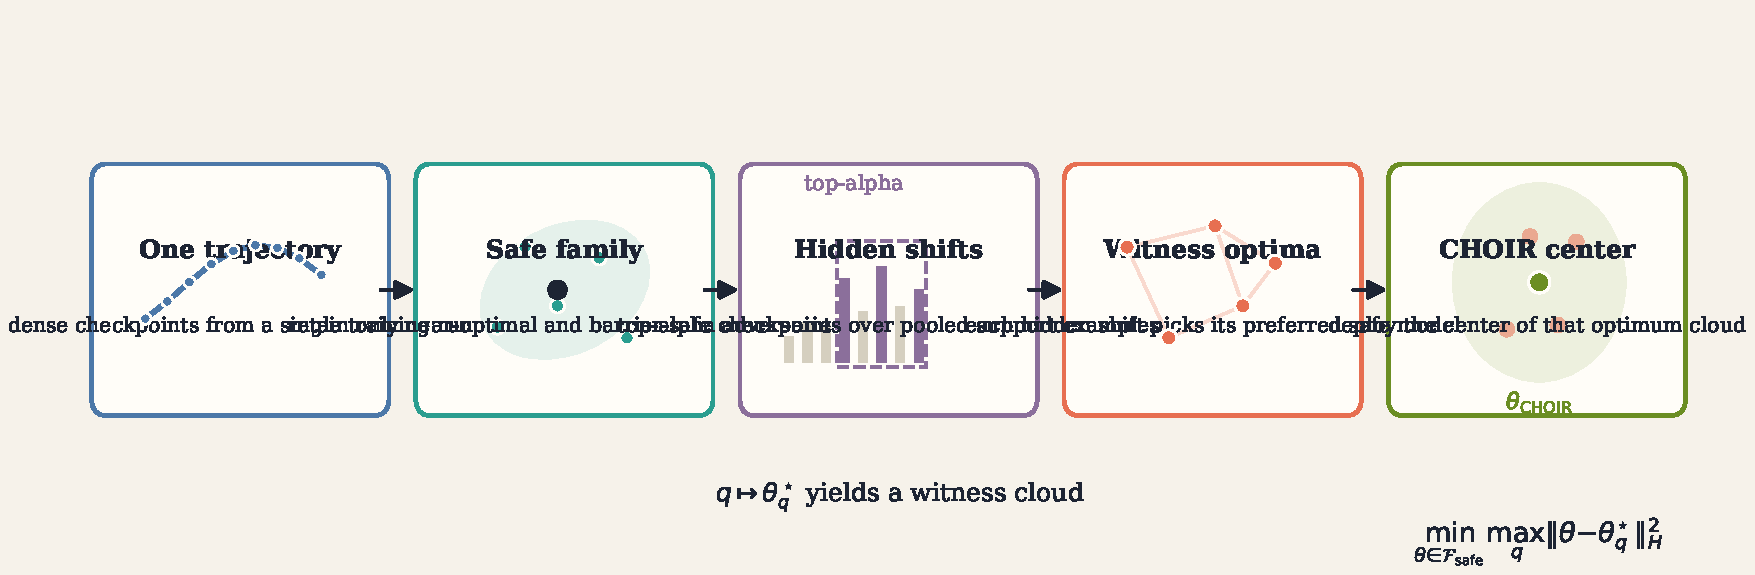
\includegraphics[width=\linewidth]{figures/choir_overview.pdf}
    \caption{\textbf{\choir{} at a glance.} From one dense trajectory, we build a safe soup family, use a finite probe set to generate active hidden shifts, compute the safe optimum preferred by each hidden shift, and deploy the center of that witness cloud.}
    \label{fig:overview}
\end{figure}

\section{Related Work}

\paragraph{Single-run post-hoc DG.}
\swad{} established flat-minima-oriented checkpoint averaging as a serious DG strategy \citep{cha2021swad}. EoA studied single-run moving averages and also heavier ensembles of averages across runs \citep{arpit2021ensemble}. These methods show that the single-run post-hoc niche is small but real. At the same time, the deployed object is still a window, a moving average, or a validation-selected average. \choir{} stays in the same post-hoc regime but studies a different selector object inside that regime.

\paragraph{Weight averaging, mode connectivity, and soups.}
Stochastic weight averaging, fast geometric ensembling, linear mode connectivity, and model soups all show that late training trajectories frequently traverse connected low-loss regions in which averaging is safe and useful \citep{izmailov2018swa,garipov2018fge,frankle2020linear,wortsman2022soups}. WiSE-FT is an especially relevant adjacent post-hoc weight-space interpolation method because it is explicitly motivated by robustness under distribution shift without adding inference-time cost \citep{wortsman2022wiseft}. \diwa{} adds an \ood{} decomposition that explains why diversity and locality jointly matter for weight averaging \citep{rame2022diwa}. \choir{} uses these works as infrastructure: a safe pool defines the feasible family. Its novelty is not another averaging heuristic inside that family, but centering the hidden-shift optima that live inside it.

\paragraph{Distributional robustness, hidden subpopulations, and regret.}
The capped source-supported shift family we use is closely related to distributionally robust optimization and worst-case subpopulation evaluation \citep{duchi2016fdiv,duchi2021learning,li2021worstcase}. Fairness without demographics and group-robust learning give additional evidence that adversarial reweightings can protect latent subpopulations without requiring observed group identities \citep{hashimoto2018fairness,lahoti2020fairness,sagawa2020groupdro}. There is also adjacent post-hoc robustness work for prior or group-prior shift \citep{wei2023priorshift}. Our objective is closer in spirit to minimax regret under shift \citep{agarwal2022mro}: the final model should remain close to what each hidden shift would ideally want, not merely obtain a low average score under one proxy.

\paragraph{Influence, local shift sensitivity, and anchor-style robustness.}
Influence functions show how sample reweightings perturb learned parameters \citep{koh2017influence}. Tangent Prop is the classical invariant-learning analogue in input space \citep{simard1991tangent}. Anchor regression shows that robustness penalties can be derived from structured shift models instead of added heuristically \citep{rothenhausler2021anchor}. \choir{} inherits the same philosophy, but its nuisance object is the empirical distribution over source support points rather than an observed domain label or an exogenous anchor variable.

\paragraph{Adjacent robust centrality and model merging.}
Robust statistics gives classical support for centrality beyond the arithmetic mean, such as the spatial median \citep{brown1983spatialmedian,minsker2024geomed}. Classical 1-center / minimum-enclosing-ball geometry is also directly relevant to the \choir{} center objective \citep{megiddo1983linear,welzl1991smallest}. Recent model-merging work explores geometric-median-style aggregation of task vectors \citep{gupta2024geomtask}. We take this adjacent literature seriously. It is exactly why this paper does \emph{not} claim that robust centrality itself is new. The novelty claim is narrower: the centered object is the \emph{hidden-shift optimum cloud extracted from a single DG trajectory}, which is different from the raw checkpoint cloud or a task-vector cloud.

\section{Problem Setup}
\label{sec:setup}

We assume a dense checkpoint bank
\[
\cC_0 = \braces{\theta_1,\ldots,\theta_T} \subset \RR^d
\]
produced by a single source-only training run. Post-hoc selection uses two pooled labeled source holdout splits:
\begin{itemize}[leftmargin=1.4em]
    \item a \emph{validation split} \(\cV\), used only to construct a safe checkpoint family, and
    \item a \emph{support split} \(\cU = \braces{(x_i,y_i)}_{i=1}^n\), used only to define hidden-shift objectives.
\end{itemize}
No source-domain labels are used after training.

\subsection{Safe checkpoint family}

For checkpoint \(\theta_t\), let
\[
\widehat L_{\cV}(\theta_t)
\triangleq
\frac{1}{|\cV|}
\sum_{(x,y)\in\cV}
-\log \max\braces{p_{\theta_t}(x)_y,\varepsilon_p}
\]
be the clipped pooled validation loss, where \(p_{\theta_t}(x)\) is the predicted class probability vector and \(\varepsilon_p \in (0,1)\) is a numerical floor.

Choose the anchor checkpoint
\[
a \in \argmin_{1\le t\le T}\widehat L_{\cV}(\theta_t).
\]
For a fixed interpolation grid \(\cA \subset [0,1]\), define the empirical barrier from the anchor to checkpoint \(t\) by
\[
B(t,a)
\triangleq
\max_{\lambda\in\cA}
\widehat L_{\cV}\paren{(1-\lambda)\theta_a + \lambda \theta_t}
-
\max\braces{\widehat L_{\cV}(\theta_a), \widehat L_{\cV}(\theta_t)}.
\]
The retained safe checkpoint set is
\begin{equation}
\cC
\triangleq
\braces{
t :
\widehat L_{\cV}(\theta_t)\le \widehat L_{\cV}^\star + \varepsilon,
\;
B(t,a)\le \tau
},
\qquad
\widehat L_{\cV}^\star = \min_t \widehat L_{\cV}(\theta_t).
\label{eq:safe_pool}
\end{equation}

The associated safe soup family is
\begin{equation}
\cF_{\safe}
\triangleq
\conv\braces{\theta_t : t\in\cC}.
\label{eq:safe_family}
\end{equation}
This paper does not claim that Eq.~\eqref{eq:safe_pool} is the only valid pool constructor. We only require a nonempty compact convex family \(\cF_{\safe}\); Eq.~\eqref{eq:safe_pool} is the concrete default because it matches the standard post-hoc DG workflow and the safe-basin intuition.

\subsection{Hidden-shift family}

On the support split \(\cU\), define the clipped per-example loss
\[
\loss_i(\theta)
\triangleq
-\log \max\braces{p_{\theta}(x_i)_{y_i}, \varepsilon_p},
\qquad
1\le i\le n.
\]
For a reweighting vector \(q\in\simplex^n\), define the reweighted empirical loss
\begin{equation}
\widehat L_q(\theta)
\triangleq
\sum_{i=1}^{n} q_i \loss_i(\theta).
\label{eq:weighted_loss}
\end{equation}

Fix \(\alpha\in(0,1]\) such that \(k=\alpha n\in\mathbb N\). The hidden-shift family is the capped simplex
\begin{equation}
\cQ_\alpha^n
\triangleq
\braces{
q\in\simplex^n :
q_i \le \frac{1}{k}\ \text{for all } i
}.
\label{eq:capped_simplex}
\end{equation}
This family encodes source-supported hidden subpopulations of size at least \(\alpha n\): the adversary may concentrate mass on any sufficiently large subset but not on a vanishing number of support points.

\begin{proposition}[Top-\(\alpha\) and empirical-\(\CVaR\) characterization]
\label{prop:topalpha}
Let \(a\in\RR^n\), let \(a_{(1)}\ge \cdots \ge a_{(n)}\) denote the decreasing rearrangement of its coordinates, and let \(k=\alpha n\in\mathbb N\). Then
\begin{equation}
\max_{q\in \cQ_\alpha^n} \sum_{i=1}^{n} q_i a_i
=
\frac{1}{k}\sum_{j=1}^{k} a_{(j)}
=
\min_{\tau\in\RR}
\braces{
\tau + \frac{1}{k}\sum_{i=1}^{n} (a_i-\tau)_+
}.
\label{eq:cvar_identity}
\end{equation}
Moreover, every extreme point of \(\cQ_\alpha^n\) is the uniform distribution on a subset of size \(k\).
\end{proposition}

Proposition~\ref{prop:topalpha} is crucial because it turns hidden shifts into concrete objects. For any probe model \(\theta\), its worst hidden shift is just the uniform distribution on its top-\(k\) support losses.

\begin{figure}[t]
    \centering
    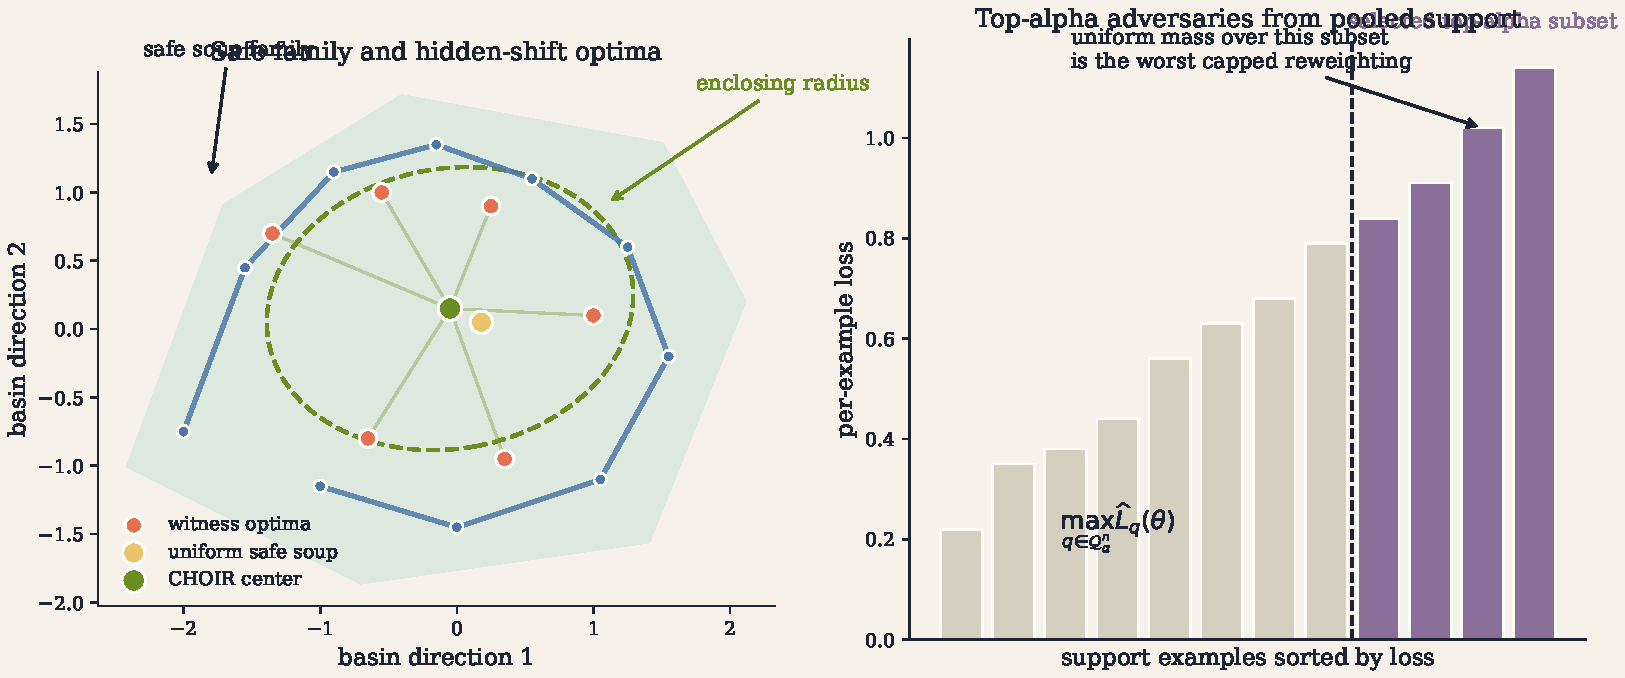
\includegraphics[width=\linewidth]{figures/choir_2d_geometry.pdf}
    \caption{\textbf{2D geometric intuition.} Left: a safe soup family with several hidden-shift optima \(w_q^\star\), the uniform-safe baseline, and the \choir{} center. Right: probe-induced top-\(\alpha\) adversaries focus on the worst \(\alpha\)-fraction of support examples for each probe model.}
    \label{fig:geometry2d}
\end{figure}

\section{The Method}
\label{sec:method}

\subsection{Probe-induced active reweightings}

\choir{} does not need to optimize over all of \(\cQ_\alpha^n\) directly. It starts from a finite probe family
\[
\cP \subset \cF_{\safe}.
\]
The default choice is
\[
\cP_{\mathrm{default}}
=
\braces{
\theta_a,\;
\bar{\theta}_{\mathrm{unif}},\;
\theta_t : t\in\cC
},
\qquad
\bar{\theta}_{\mathrm{unif}}
=
\frac{1}{|\cC|}\sum_{t\in\cC}\theta_t.
\]
For each probe \(p\in\cP\), define the adversarial reweighting
\[
q_p \in \argmax_{q\in\cQ_\alpha^n} \widehat L_q(p).
\]
By Proposition~\ref{prop:topalpha}, \(q_p\) is a top-\(\alpha\) support subset for probe \(p\). The active family is the deduplicated set
\begin{equation}
\cQ_{\act}
\triangleq
\braces{q_p : p\in\cP}.
\label{eq:active_set}
\end{equation}
The default probe-induced active family is a heuristic coverage set. Later exact finite-set results apply to whatever finite \(\cQ_{\act}\) is supplied, whereas the \(\varepsilon\)-net approximation result only applies when that finite set comes with an explicit coverage guarantee.

\subsection{Witness optima}

For each active hidden shift \(q\in\cQ_{\act}\), define its safe optimum
\begin{equation}
\theta_q^\star
\in
\argmin_{\theta\in\cF_{\safe}}
\widehat L_q(\theta).
\label{eq:witness_def}
\end{equation}
The witness cloud is
\[
\cW^\star \triangleq \braces{\theta_q^\star : q\in\cQ_{\act}}.
\]

Equation~\eqref{eq:witness_def} is the point at which \choir{} diverges from existing scalar post-hoc objectives. We do not ask which model wins one universal scoreboard. We ask what each plausible hidden shift would choose for itself inside the same safe family.

\paragraph{Practical witness solver.}
The convex-hull representation in checkpoint coefficients is generally redundant: if the safe checkpoints are affinely dependent, then strong convexity in the raw simplex coefficients is impossible along null directions that leave the same model unchanged. For theory we therefore reduce to affine-hull coordinates before stating any witness-oracle rate.

Fix any \(\theta_0\in\cF_{\safe}\), let \(r=\dim \aff(\cF_{\safe})\), and let \(U\in\RR^{d\times r}\) have full column rank with
\[
\aff(\cF_{\safe}) = \theta_0 + \operatorname{range}(U).
\]
Define the reduced feasible set and reduced metric
\[
\cZ_{\safe}
\triangleq
\braces{z\in\RR^r : \theta_0 + Uz \in \cF_{\safe}}.
\]
For fixed \(q\), define the reduced witness objective
\[
h_q(z)
\triangleq
\widehat L_q(\theta_0 + Uz).
\]
Then Eq.~\eqref{eq:witness_def} is equivalent to minimizing \(h_q\) on \(\cZ_{\safe}\). Practical code may still optimize over checkpoint coefficients or directly over soups, but the nondegenerate witness theorem is stated in these reduced coordinates.

\begin{theorem}[Linear convergence of the reduced-coordinate witness oracle]
\label{thm:witness_pgd}
Fix \(q\in\cQ_{\act}\). Suppose \(h_q\) extends to a twice continuously differentiable function on an open neighborhood of \(\cZ_{\safe}\) and satisfies
\[
\mu_q I \preceq \nabla^2 h_q(z) \preceq L_q I
\qquad
\forall z \text{ in that neighborhood},
\]
where \(0<\mu_q\le L_q\). Let
\[
z_q^\star\in\argmin_{z\in\cZ_{\safe}} h_q(z),
\qquad
\theta_q^\star = \theta_0 + U z_q^\star,
\]
and consider projected gradient descent
\begin{equation}
z^{(s+1)}
=
\Pi_{\cZ_{\safe}}
\paren{
z^{(s)} - \eta \nabla h_q\paren{z^{(s)}}
},
\qquad s=0,1,2,\ldots
\label{eq:witness_pgd}
\end{equation}
with any step size \(\eta\in\paren{0,\frac{2}{L_q}}\). Then
\begin{equation}
\norm{z^{(s+1)}-z_q^\star}_2
\le
\gamma_q(\eta)\,
\norm{z^{(s)}-z_q^\star}_2,
\qquad
\gamma_q(\eta)
\triangleq
\max\braces{\abs{1-\eta\mu_q},\abs{1-\eta L_q}} < 1.
\label{eq:witness_pgd_rate}
\end{equation}
Consequently,
\[
\norm{z^{(s)}-z_q^\star}_2
\le
\gamma_q(\eta)^s
\norm{z^{(0)}-z_q^\star}_2,
\]
and the corresponding witness iterate \(\theta^{(s)}_q = \theta_0 + U z^{(s)}\) converges linearly to \(\theta_q^\star\). The optimal fixed step size is \(\eta^\star = \frac{2}{\mu_q + L_q}\), which yields
\[
\gamma_q(\eta^\star)
=
\frac{L_q-\mu_q}{L_q+\mu_q}.
\]
\end{theorem}

Theorem~\ref{thm:witness_pgd} is a standard convex-optimization guarantee for the reduced-coordinate witness oracle. We include it only to make the oracle assumptions explicit and to justify the optimization subroutine used in the practical soup variant. The affine reduction is important: without it, redundant simplex coefficients generically destroy the strong-convexity premise.

\subsection{The \choir{} center}

Let \(H\in\RR^{d\times d}\) be any symmetric positive definite local basin metric. The default choices are \(H=I_d\) or a regularized empirical Fisher metric computed around the uniform-safe soup. Define
\[
\norm{v}_H^2 \triangleq v^\top H v.
\]
Given the affine-hull basis \(U\) introduced above, write
\[
H_U \triangleq U^\top H U \succ 0.
\]
The \choir{} center is
\begin{equation}
\theta_{\choir}
\in
\argmin_{\theta\in\cF_{\safe}}
\max_{q\in\cQ_{\act}}
\norm{\theta-\theta_q^\star}_{H}^{2}.
\label{eq:choir_center}
\end{equation}
The objective in Eq.~\eqref{eq:choir_center} is a classical minimum-enclosing-ball / 1-center problem in the \(H\)-metric, restricted to the safe family \citep{megiddo1983linear,welzl1991smallest}.

\begin{theorem}[Existence, uniqueness, and dual characterization]
\label{thm:center_dual}
Let \(\cW=\braces{w_1,\ldots,w_M}\subset \cF_{\safe}\) be a nonempty finite witness cloud and define
\[
J_{\cW}(\theta)
\triangleq
\max_{1\le j\le M}\norm{\theta-w_j}_H^2.
\]
Then:
\begin{enumerate}[label=(\alph*),leftmargin=1.4em]
    \item \(J_{\cW}\) has a unique minimizer \(\theta_{\cW}^\star\) on \(\cF_{\safe}\).
    \item The minimizer belongs to \(\conv(\cW)\), so minimizing over \(\cF_{\safe}\) is equivalent to minimizing over \(\conv(\cW)\).
    \item The optimum admits the exact dual characterization
    \begin{equation}
    \min_{\theta\in\cF_{\safe}} J_{\cW}(\theta)
    =
    \max_{\lambda\in\simplex^{M}}
    \sum_{j=1}^{M}\lambda_j
    \norm{w_j-\bar w_\lambda}_H^2,
    \qquad
    \bar w_\lambda = \sum_{j=1}^{M}\lambda_j w_j.
    \label{eq:center_dual}
    \end{equation}
    Every maximizing \(\lambda^\star\) satisfies \(\theta_{\cW}^\star=\bar w_{\lambda^\star}\).
\end{enumerate}
\end{theorem}

Theorem~\ref{thm:center_dual} means the \choir{} center is itself a barycenter of witness optima. The underlying 1-center geometry is classical; the point here is its DG instantiation on the hidden-shift witness cloud. Since every witness optimum is a safe soup, the final model is also a safe soup.

\begin{corollary}[Sparse deployability]
\label{cor:sparse}
Let \(d_{\aff}\) be the affine dimension of \(\cW^\star\). Then some optimal \choir{} center can be represented as a convex combination of at most \(d_{\aff}+1\) witness optima. If each witness optimum uses at most \(s\) safe checkpoints in its own soup representation, then some optimal \choir{} deployment uses at most \(s(d_{\aff}+1)\) safe checkpoints.
\end{corollary}

\subsection{Exact center solver}

For a finite witness cloud \(\cW\), Eq.~\eqref{eq:choir_center} can be written as the convex program
\begin{equation}
\begin{aligned}
\min_{\theta\in\cF_{\safe},\ \rho\in\RR}\quad & \rho \\
\text{s.t.}\quad &
\norm{\theta-w}_H^2 \le \rho
\qquad \forall w\in\cW.
\end{aligned}
\label{eq:master_qp}
\end{equation}
When \(\cW\) is large, \choir{} may solve Eq.~\eqref{eq:master_qp} by constraint generation. In the default finite-active-set pipeline, the full witness cloud is already computed explicitly, so the wrapper below is best read as an exact-QP template rather than as a hidden oracle story.

\begin{algorithm}[t]
\caption{\choir{} with probe-induced active reweightings}
\label{alg:choir}
\begin{algorithmic}[1]
\Require checkpoint bank \(\cC_0\), validation split \(\cV\), support split \(\cU\), thresholds \(\varepsilon,\tau\), mass level \(\alpha\), probe family \(\cP\), metric \(H\)
\State Build safe checkpoint set \(\cC\) by Eq.~\eqref{eq:safe_pool} and safe soup family \(\cF_{\safe}=\conv\braces{\theta_t:t\in\cC}\)
\State Construct \(\cQ_{\act}\) by Eqs.~\eqref{eq:active_set} and \eqref{eq:cvar_identity}
\ForAll{\(q\in\cQ_{\act}\)}
    \State Compute witness optimum \(\theta_q^\star \in \argmin_{\theta\in\cF_{\safe}} \widehat L_q(\theta)\)
\EndFor
\State Initialize working witness set \(\cW_1\) with any one witness
\For{\(k=1,2,\ldots\)}
    \State Solve the master program Eq.~\eqref{eq:master_qp} using only constraints \(w\in\cW_k\), obtaining \((\theta_k,\rho_k)\)
    \State Find a most violated witness \(w_k \in \argmax_{w\in\cW^\star}\norm{\theta_k-w}_H^2\)
    \If{\(\norm{\theta_k-w_k}_H^2 \le \rho_k\)}
        \State \Return \(\theta_k\)
    \Else
        \State \(\cW_{k+1}\gets \cW_k \cup \braces{w_k}\)
    \EndIf
\EndFor
\end{algorithmic}
\end{algorithm}

\begin{theorem}[Finite termination of Algorithm~\ref{alg:choir}]
\label{thm:finite_termination}
Algorithm~\ref{alg:choir} terminates in at most \(\abs{\cW^\star}\) iterations and returns the exact solution of Eq.~\eqref{eq:choir_center}.
\end{theorem}

Theorem~\ref{thm:finite_termination} is a finite-set bookkeeping fact for the exact center solver, included for completeness rather than as a novelty claim.

\section{Theory}
\label{sec:theory}

\subsection{Why centering the optimum cloud controls hidden-shift regret}

The key term in \choir{} is the squared distance to each witness optimum. The next results are deliberately stated for an idealized reference hidden-shift family: they assume that the full witness map exists with affine-hull relative-interior optima and controlled local curvature. Their role is to justify why active-set coverage matters, not to claim a global theorem about arbitrary deep-network loss surfaces.

\begin{assumption}[Reference-family relative-interior witness optima]
\label{ass:interior}
Fix \(\theta_0\in\cF_{\safe}\), let \(U\in\RR^{d\times r}\) have full column rank with \(\aff(\cF_{\safe})=\theta_0+\operatorname{range}(U)\), and define
\[
\cZ_{\safe}
=
\braces{z\in\RR^r : \theta_0 + Uz \in \cF_{\safe}}.
\]
For every \(q\in\cQ_\alpha^n\), the reduced witness problem admits an optimum \(z_q^\star\in\ri(\cZ_{\safe})\) with
\[
\theta_q^\star = \theta_0 + U z_q^\star,
\qquad
h_q(z)=\widehat L_q(\theta_0+Uz),
\]
and \(h_q\) is differentiable at \(z_q^\star\) with
\[
\nabla h_q(z_q^\star)=0.
\]
Equivalently,
\[
U^\top \nabla \widehat L_q(\theta_q^\star)=0.
\]
\end{assumption}

\begin{theorem}[Local Hessian domination implies regret domination]
\label{thm:regret_domination}
Assume Assumption~\ref{ass:interior}. Fix \(q\in\cQ_\alpha^n\). If \(\widehat L_q\) is twice continuously differentiable on an open neighborhood of \(\cF_{\safe}\) and
\begin{equation}
U^\top \nabla^2 \widehat L_q(\theta_0+Uz) U \preceq \beta_q U^\top H U
\qquad
\forall z\in\cZ_{\safe},
\label{eq:hessian_domination}
\end{equation}
then for every \(\theta\in\cF_{\safe}\),
\begin{equation}
\widehat L_q(\theta)-\widehat L_q(\theta_q^\star)
\le
\frac{\beta_q}{2}\norm{\theta-\theta_q^\star}_{H}^{2}.
\label{eq:regret_domination}
\end{equation}
\end{theorem}

Theorem~\ref{thm:regret_domination} is an exact derivation, not a sketch. The squared \(H\)-distance in Eq.~\eqref{eq:choir_center} is the local upper model naturally induced by the hidden-shift Hessians.

\begin{corollary}[Worst-case regret bound for ideal \choir{}]
\label{cor:ideal_regret}
Let
\[
R_\act^2
\triangleq
\min_{\theta\in\cF_{\safe}}
\max_{q\in\cQ_{\act}}
\norm{\theta-\theta_q^\star}_H^2.
\]
Under the assumptions of Theorem~\ref{thm:regret_domination} for all \(q\in\cQ_{\act}\), with \(\beta_{\act,\max}=\max_{q\in\cQ_{\act}}\beta_q\), the ideal \choir{} center satisfies
\[
\max_{q\in\cQ_{\act}}
\Reg_q(\theta_{\choir})
\le
\frac{\beta_{\act,\max}}{2} R_\act^2,
\qquad
\Reg_q(\theta)
\triangleq
\widehat L_q(\theta)-\widehat L_q(\theta_q^\star).
\]
\end{corollary}

\subsection{Witness stability and active-set approximation}

The next results quantify the price of not optimizing over the full capped simplex.

\begin{assumption}[Local strong convexity and bounded per-example gradients]
\label{ass:strong}
There exists \(m>0\) and \(G_0>0\) such that:
\begin{enumerate}[label=(\roman*),leftmargin=1.4em]
    \item for every \(q\in\cQ_\alpha^n\), the reduced objective \(h_q(z)=\widehat L_q(\theta_0+Uz)\) is \(m\)-strongly convex on \(\cZ_{\safe}\) with respect to the \(H_U\)-norm, and
    \item for every \(i\in\braces{1,\ldots,n}\) and \(\theta\in\cF_{\safe}\),
    \[
    \norm{U^\top \nabla \loss_i(\theta)}_{H_U^{-1}} \le G_0.
    \]
\end{enumerate}
\end{assumption}

\begin{theorem}[Lipschitz witness map]
\label{thm:witness_lipschitz}
Under Assumptions~\ref{ass:interior} and \ref{ass:strong}, the full witness map \(q\mapsto \theta_q^\star\) is Lipschitz:
\begin{equation}
\norm{\theta_q^\star-\theta_{q'}^\star}_H
\le
\frac{G_0}{m}\norm{q-q'}_1
\qquad
\forall q,q'\in\cQ_\alpha^n.
\label{eq:witness_lipschitz}
\end{equation}
\end{theorem}

\begin{theorem}[Witness-cloud perturbation bound]
\label{thm:hausdorff}
Let \(\cW,\widetilde{\cW}\subset\cF_{\safe}\) be two nonempty compact witness sets, define
\[
J_{\cW}(\theta)
\triangleq
\sup_{w\in\cW}\norm{\theta-w}_H^2,
\qquad
J_{\widetilde{\cW}}(\theta)
\triangleq
\sup_{w\in\widetilde{\cW}}\norm{\theta-w}_H^2,
\]
and write
\[
\eta \triangleq \Haus_H(\cW,\widetilde{\cW}),
\qquad
D \triangleq
\sup_{\theta\in\cF_{\safe},\; w\in\cW\cup\widetilde{\cW}}
\norm{\theta-w}_H.
\]
If \(\widetilde\theta^\star\) is the \choir{} center of \(\widetilde{\cW}\), then
\begin{align}
\abs{
\min_{\theta\in\cF_{\safe}} J_{\cW}(\theta)
-
\min_{\theta\in\cF_{\safe}} J_{\widetilde{\cW}}(\theta)
}
&\le 2D\eta + \eta^2,
\label{eq:value_perturb}\\
J_{\cW}(\widetilde\theta^\star)
&\le
\min_{\theta\in\cF_{\safe}} J_{\widetilde{\cW}}(\theta) + 2D\eta + \eta^2.
\label{eq:policy_perturb}
\end{align}
\end{theorem}

\begin{corollary}[Approximation by an externally supplied \(\varepsilon\)-net active set]
\label{cor:epsnet}
Assume the conditions of Theorems~\ref{thm:regret_domination}, \ref{thm:witness_lipschitz}, and \ref{thm:hausdorff}. Let \(\cQ_{\act}\subset\cQ_\alpha^n\) be an \(\varepsilon\)-net in \(\ell_1\), and let \(\theta_{\choir,\act}\) denote the \choir{} center computed from \(\cQ_{\act}\). Then
\[
\beta_{\full,\max}
\triangleq
\sup_{q\in\cQ_\alpha^n}\beta_q
\]
is assumed finite, and
\[
\sup_{q\in\cQ_\alpha^n}
\Reg_q(\theta_{\choir,\act})
\le
\frac{\beta_{\full,\max}}{2}
\paren{
R_\act^2 + 2D\frac{G_0}{m}\varepsilon + \frac{G_0^2}{m^2}\varepsilon^2
}.
\]
\end{corollary}

Corollary~\ref{cor:epsnet} does \emph{not} certify that the default probe-induced active set in Eq.~\eqref{eq:active_set} is an \(\varepsilon\)-net. It states what would follow for any finite active set equipped with an external coverage guarantee or a certified densification procedure.

\begin{corollary}[Approximation by practical witness oracles]
\label{cor:oracle}
Suppose the practical witness oracle returns \(\widetilde\theta_q\in\cF_{\safe}\) satisfying
\[
\norm{\widetilde\theta_q-\theta_q^\star}_H \le \delta
\qquad
\forall q\in\cQ_{\act}.
\]
Let \(\widetilde\theta_{\choir}\) be the center computed from the approximate witness cloud \(\widetilde{\cW}\triangleq\braces{\widetilde\theta_q:q\in\cQ_{\act}}\). Then
\[
\beta_{\act,\max}
\triangleq
\max_{q\in\cQ_{\act}}\beta_q
\]
and
\[
\max_{q\in\cQ_{\act}}
\Reg_q(\widetilde\theta_{\choir})
\le
\frac{\beta_{\act,\max}}{2}\paren{R_\act^2 + 2D\delta + \delta^2 }.
\]
\end{corollary}

Corollary~\ref{cor:oracle} is the bridge to the one-shot practical version. The first empirical implementation can restrict the witness oracle in Eq.~\eqref{eq:witness_def} to the finite checkpoint bank itself. The theory then applies through the induced approximation error \(\delta\).

\begin{figure}[t]
    \centering
    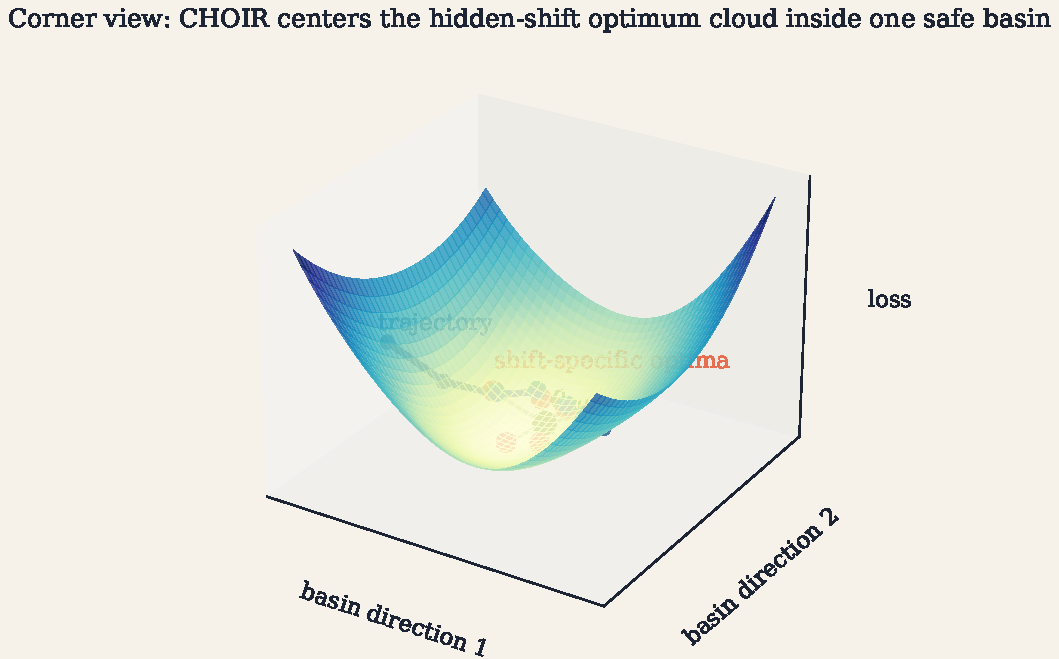
\includegraphics[width=\linewidth]{figures/choir_3d_cloud.pdf}
    \caption{\textbf{3D corner view.} A safe basin extracted from one training trajectory is shown as a curved low-loss region. Different hidden shifts prefer different witness optima inside that basin, and \choir{} centers that optimum cloud rather than choosing the loudest witness.}
    \label{fig:geometry3d}
\end{figure}

\section{Discussion of Assumptions}
\label{sec:assumptions}

\paragraph{Why we use the capped simplex.}
Equation~\eqref{eq:capped_simplex} is a standard DRO-style, source-supported hidden-shift family. We use it because it simultaneously (i) stays entirely on source support, (ii) explicitly protects large hidden subpopulations, and (iii) admits the exact top-\(\alpha\) and empirical-\(\CVaR\) characterization of Proposition~\ref{prop:topalpha}. That last property is what makes the probe-induced active set deterministic and computationally manageable.

\paragraph{Why local curvature is acceptable here.}
Theorem~\ref{thm:regret_domination} is explicitly local and idealized. It does not claim global convexity in network weight space. It only claims that once a safe family has been isolated, hidden-shift regret can be upper-bounded by a quadratic form if the hidden-shift Hessians are dominated by the chosen basin metric \(H\) on the affine hull of that family. The same honesty applies to the full-family stability results: they require relative-interior witness optima and controlled curvature on the reference hidden-shift family, and should be read as justification for the active-set design rather than as a literal theorem about arbitrary deep-network weight space.

\paragraph{What the smoothness assumptions do and do not cover.}
The benchmark architecture we target is typically a ReLU-based ResNet-50, so the \(C^2\) assumptions used in Theorems~\ref{thm:witness_pgd} and \ref{thm:regret_domination} should be read as idealized local smooth analysis, not as literal statements about every activation boundary of a raw ReLU network. In practice this can be interpreted as a statement about neighborhoods that do not cross activation-pattern changes, about smoothed surrogates, or about almost-everywhere Hessian surrogates. We do not claim otherwise.

\paragraph{Where the theory can fail.}
There are three primary failure modes:
\begin{enumerate}[leftmargin=1.4em]
    \item \textbf{Witness collapse.} If all \(q\in\cQ_{\act}\) choose nearly the same optimum, \choir{} collapses to the obvious baseline. This is not a bug; it means the hidden-shift optimum cloud is tiny.
    \item \textbf{Empirical safe-set misspecification.} The \choir{} optimizer itself never leaves \(\cF_{\safe}\); the real risk is that the empirically constructed \(\cF_{\safe}\) may fail to track the truly safe basin. In that case every post-hoc method restricted to \(\cF_{\safe}\), including \choir{}, can inherit the misspecification.
    \item \textbf{Bad active-set coverage.} If the probe-induced active set misses important regions of \(\cQ_\alpha^n\), then Corollary~\ref{cor:epsnet} does not apply, and the default active-set construction should be viewed as heuristic rather than certified coverage.
\end{enumerate}

\section{Experimental Protocol and Published Benchmark Context}
\label{sec:experiments}

This section is complete as an evaluation protocol, but every new \choir{} number is intentionally left as \TBD{} until the actual experiments are run.

\subsection{Benchmarks, backbone, and metrics}

We will evaluate on the five standard real-image DomainBed datasets most commonly used in published DG comparisons \citep{gulrajani2021domainbed}: PACS, VLCS, OfficeHome, TerraIncognita, and DomainNet. DomainBed contains additional benchmarks; we focus here on the standard real-image subset because that is the comparison regime used by the published post-hoc results reported below. The default backbone is the ImageNet-pretrained ResNet-50 used in the most common published DG comparisons. We will report per-dataset average accuracy and the overall average across the five datasets, together with standard errors over repeated trials. Any deviation from this protocol will be stated explicitly in the final camera-ready version.

\subsection{Baselines}

The comparison set will include:
\begin{itemize}[leftmargin=1.4em]
    \item the base \erm{} checkpoint,
    \item the uniform safe soup baseline,
    \item current post-hoc DG baselines such as \swad{},
    \item the narrow \choir{} checkpoint-only practical variant,
    \item the full \choir{} safe-soup variant,
    \item ablations that remove active reweighting, witness centering, or the \(H\)-metric.
\end{itemize}

\subsection{Published benchmark context}

Table~\ref{tab:published_context} records exact published averages from earlier work. The settings are not perfectly identical, so the table should be read as context rather than as an apples-to-apples leaderboard.

\begin{table}[t]
    \centering
    \caption{\textbf{Published benchmark context from prior work.} These are exact published averages copied from the cited papers. The settings differ, so this table is reference context, not a direct leaderboard for \choir{}.}
    \label{tab:published_context}
    \small
    \setlength{\tabcolsep}{5pt}
    \begin{adjustbox}{max width=\linewidth}
    \begin{tabular}{@{}lp{5.4cm}ll@{}}
        \toprule
        Method & Setting & Single run? & Published Avg. \\
        \midrule
        \erm{} \citep{cha2021swad} & DomainBed ResNet-50 & N/A & 63.3 \\
        \swad{} \citep{cha2021swad} & DomainBed ResNet-50 & yes & 66.9 \\
        EoA \citep{arpit2021ensemble} & pre-trained ResNet-50, strongest reported setting & partly & 68.0 \\
        \diwa{}$^\dagger$ \citep{rame2022diwa} & LP init, multi-run, \(M=60\) & no & 68.0 \\
        \miro{} + \swad{} \citep{cha2022miro} & ResNet-50 + \swad{} & no & 68.1 \\
        \bottomrule
    \end{tabular}
    \end{adjustbox}
\end{table}

\begin{table}[t]
    \centering
    \caption{\textbf{Published dataset-wise context from prior work.} Only rows whose exact dataset-wise values were independently verified from the cited paper sources are included here. Rows corresponding to the upcoming \choir{} run remain intentionally \TBD{}.}
    \label{tab:published_dataset_context}
    \begin{tabular}{lcccccc}
        \toprule
        Method & PACS & VLCS & OfficeHome & TerraIncognita & DomainNet & Avg. \\
        \midrule
        \erm{} \citep{cha2021swad} & 85.5 & 77.5 & 66.5 & 46.1 & 40.9 & 63.3 \\
        \swad{} \citep{cha2021swad} & 88.1 & 79.1 & 70.6 & 50.0 & 46.5 & 66.9 \\
        \diwa{}$^\dagger$ \citep{rame2022diwa} & 89.0 & 78.6 & 72.8 & 51.9 & 47.7 & 68.0 \\
        \miro{} + \swad{} \citep{cha2022miro} & 88.4 & 79.6 & 72.4 & 52.9 & 47.0 & 68.1 \\
        \bottomrule
    \end{tabular}
\end{table}

\subsection{Main results table}

\begin{table}[t]
    \centering
    \caption{\textbf{Planned run-specific results.} Only rows tied to the upcoming \choir{} run remain \TBD{}.}
    \label{tab:main_results}
    \scriptsize
    \begin{adjustbox}{width=\linewidth,center}
    \begin{tabular}{lcccccc}
        \toprule
        Method & PACS & VLCS & OfficeHome & TerraIncognita & DomainNet & Avg. \\
        \midrule
        Base \erm{} (this run) & \TBD{} & \TBD{} & \TBD{} & \TBD{} & \TBD{} & \TBD{} \\
        Uniform safe soup (run) & \TBD{} & \TBD{} & \TBD{} & \TBD{} & \TBD{} & \TBD{} \\
        \swad{} (this run) & \TBD{} & \TBD{} & \TBD{} & \TBD{} & \TBD{} & \TBD{} \\
        \choir{}-Checkpoint & \TBD{} & \TBD{} & \TBD{} & \TBD{} & \TBD{} & \TBD{} \\
        \choir{}-Soup & \TBD{} & \TBD{} & \TBD{} & \TBD{} & \TBD{} & \TBD{} \\
        \bottomrule
    \end{tabular}
    \end{adjustbox}
\end{table}

\subsection{Ablations and diagnostics}

\begin{table}[t]
    \centering
    \caption{\textbf{Planned ablation grid.} Every entry is intentionally \TBD{} until experiments are run.}
    \label{tab:ablations}
    \begin{tabular}{ll}
        \toprule
        Ablation family & Planned values / diagnostics \\
        \midrule
        Probe family size & \TBD{} \\
        Hidden-shift mass \(\alpha\) & \TBD{} \\
        Metric \(H\) & \TBD{} \\
        Witness oracle & \TBD{} \\
        Center type & \TBD{} \\
        Safety fallback frequency & \TBD{} \\
        Witness-cloud radius & \TBD{} \\
        Active-set coverage diagnostics & \TBD{} \\
        \bottomrule
    \end{tabular}
\end{table}

\begin{figure}[t]
    \centering
    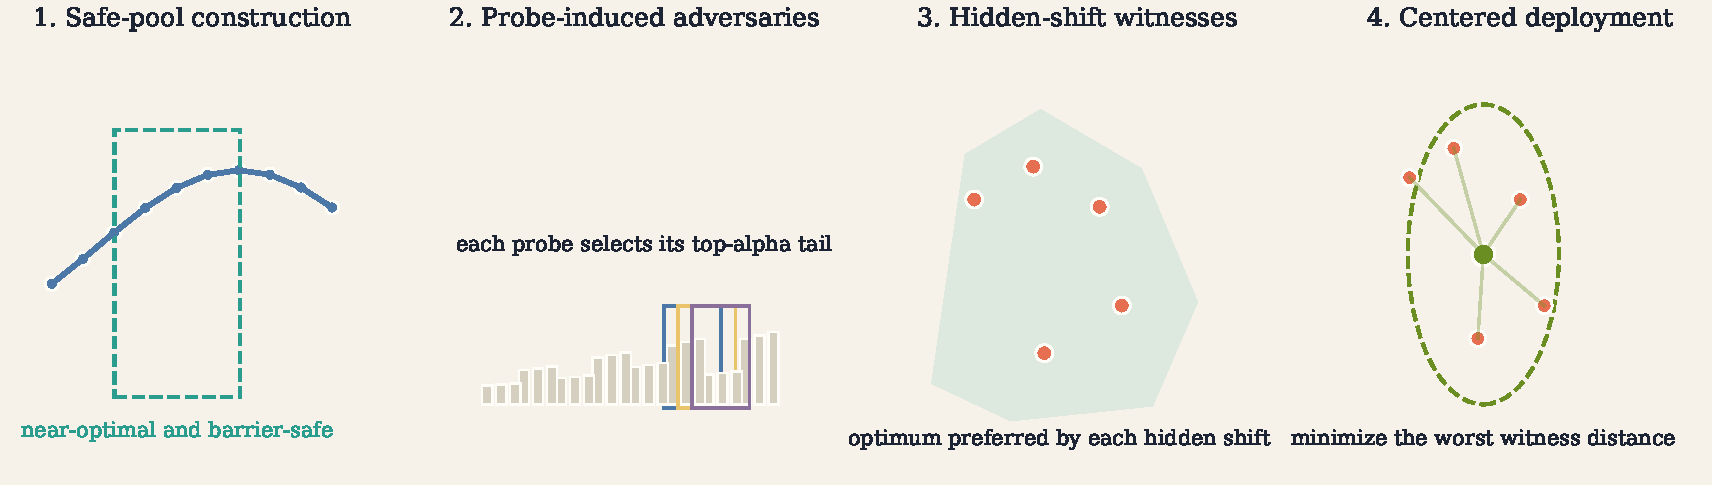
\includegraphics[width=\linewidth]{figures/choir_step_panels.pdf}
    \caption{\textbf{Visual intuition for each step.} From left to right: safe-pool construction, probe-induced adversaries, hidden-shift witness optima, and the final centered deployment.}
    \label{fig:step_panels}
\end{figure}

\section{Limitations}

\choir{} is not a claim about arbitrary \ood{} shifts. Its theorems apply only to source-supported hidden shifts and only inside an empirically safe family. If the target distribution lies far outside the source support hull, or if the safe family is itself badly misidentified, then no post-hoc selector built on that family can be expected to save the situation. The paper is also honest about the active-set issue: \choir{} only sees the hidden shifts it probes or approximates. This is why the approximation results in Section~\ref{sec:theory} are written explicitly in terms of active-set coverage and witness-oracle error.

\section{Conclusion}

\choir{} proposes a different answer to the central post-hoc DG question. Instead of asking which safe checkpoint soup wins one global score, it asks what each plausible hidden source-supported shift would choose for itself, then deploys the center of that optimum cloud. The resulting method is still single-run, still domain-label-free, still post-hoc, and still a single deployable soup at inference time. The paper provides a conditional local analysis for this narrowed version: exact hidden-shift characterization, exact center duality, finite-termination optimization, local regret domination on the affine hull of the safe family, and explicit active-set and witness-approximation bounds under strong geometric assumptions. The empirical section is deliberately unfinished only in the narrow sense required by the current project state: the protocol is complete, but every new \choir{} number remains \TBD{} until the experiments are run.

\bibliographystyle{plainnat}
\bibliography{references}

\appendix

\section{Additional Visual Intuition}

Figure~\ref{fig:active_set} gives one more visual view of the active-set construction and the relation between the hidden-shift family in reweighting space and the witness cloud in model space.

\begin{figure}[h]
    \centering
    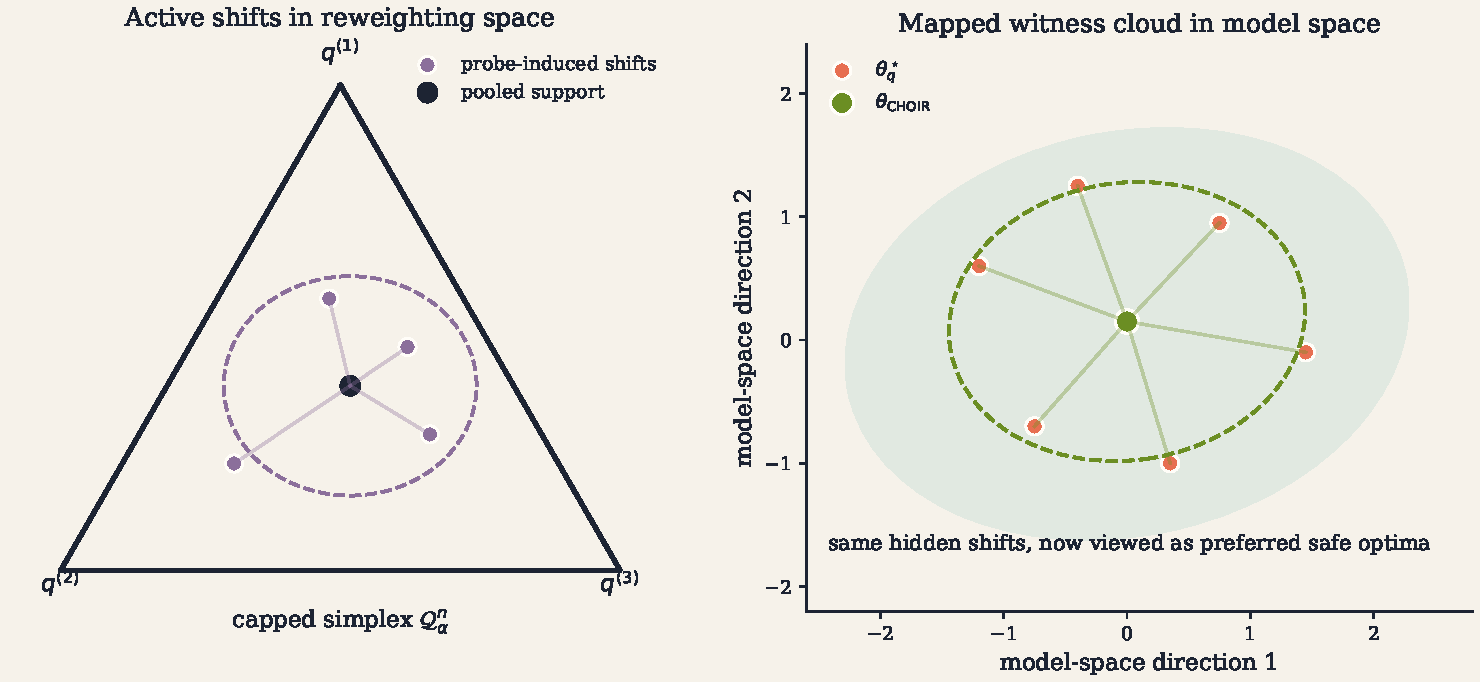
\includegraphics[width=\linewidth]{figures/choir_active_set.pdf}
    \caption{\textbf{Active-set intuition.} Left: the capped simplex in reweighting space and probe-induced hidden shifts. Right: the corresponding witness cloud in model space together with the \choir{} center and its enclosing radius.}
    \label{fig:active_set}
\end{figure}

\section{Full Proofs}

\subsection{Proof of Proposition~\ref{prop:topalpha}}

\begin{proof}
We proceed in three steps.

\paragraph{Step 1: characterize the extreme points of \(\cQ_\alpha^n\).}
Recall
\[
\cQ_\alpha^n
=
\braces{
q\in\RR^n :
q_i\ge 0,\;
\sum_{i=1}^{n} q_i = 1,\;
q_i \le \frac{1}{k}
}.
\]
Let \(q\in \cQ_\alpha^n\). Suppose there exist two distinct indices \(i\neq j\) such that
\[
0 < q_i < \frac{1}{k},
\qquad
0 < q_j < \frac{1}{k}.
\]
Choose
\[
\varepsilon
<
\min\braces{
q_i,\;
\frac{1}{k}-q_i,\;
q_j,\;
\frac{1}{k}-q_j
}.
\]
Define
\[
q^{+}= q + \varepsilon (e_i-e_j),
\qquad
q^{-}= q - \varepsilon (e_i-e_j),
\]
where \(e_i\) is the \(i\)-th standard basis vector. Then \(q^+,q^- \in \cQ_\alpha^n\), \(q=\frac{1}{2}(q^+ + q^-)\), and \(q^+\neq q^-\). Hence \(q\) is not an extreme point.

Therefore every extreme point has at most one coordinate strictly between \(0\) and \(1/k\). But the equality constraint \(\sum_i q_i = 1\) together with the upper bound \(q_i\le 1/k\) implies that at least \(k\) coordinates must be positive. Since \(k\cdot \frac{1}{k}=1\), the only way to sum to one is to have exactly \(k\) coordinates equal to \(1/k\) and the rest equal to \(0\). Thus every extreme point is the uniform distribution on some subset \(S\subseteq\braces{1,\ldots,n}\) of size \(k\).

\paragraph{Step 2: maximize a linear functional.}
Since \(q\mapsto \sum_i q_i a_i\) is linear and \(\cQ_\alpha^n\) is a compact polytope, its maximum is attained at an extreme point. By Step 1, we only need to consider vectors that place mass \(1/k\) on a subset \(S\) of size \(k\). For such a vector,
\[
\sum_{i=1}^{n} q_i a_i
=
\frac{1}{k}\sum_{i\in S} a_i.
\]
This is maximized by choosing \(S\) to contain the \(k\) largest coordinates of \(a\), hence
\[
\max_{q\in\cQ_\alpha^n}\sum_{i=1}^{n} q_i a_i
=
\frac{1}{k}\sum_{j=1}^{k} a_{(j)}.
\]

\paragraph{Step 3: empirical-\(\CVaR\) representation.}
Define
\[
\phi(\tau)
\triangleq
\tau + \frac{1}{k}\sum_{i=1}^{n} (a_i-\tau)_+.
\]
We will show
\[
\min_{\tau\in\RR}\phi(\tau)
=
\frac{1}{k}\sum_{j=1}^{k} a_{(j)}.
\]
\paragraph{Lower bound.}
For any \(\tau\in\RR\),
\[
\sum_{i=1}^{n}(a_i-\tau)_+
\ge
\sum_{j=1}^{k}(a_{(j)}-\tau),
\]
because \((a_i-\tau)_+\) dominates the contribution of the largest \(k\) coordinates. Therefore
\[
\phi(\tau)
\ge
\tau + \frac{1}{k}\sum_{j=1}^{k}(a_{(j)}-\tau)
=
\frac{1}{k}\sum_{j=1}^{k} a_{(j)}.
\]

\paragraph{Matching upper bound.}
If \(k<n\), choose any \(\tau\in[a_{(k+1)},a_{(k)}]\). Then \(a_{(j)}-\tau\ge 0\) for \(j\le k\) and \(a_{(j)}-\tau\le 0\) for \(j>k\), so
\[
\sum_{i=1}^{n}(a_i-\tau)_+
=
\sum_{j=1}^{k}(a_{(j)}-\tau),
\]
and hence
\[
\phi(\tau)
=
\frac{1}{k}\sum_{j=1}^{k} a_{(j)}.
\]
If \(k=n\), choose any \(\tau\le a_{(n)}\). Then every term is nonnegative and
\[
\phi(\tau)
=
\tau + \frac{1}{n}\sum_{i=1}^{n}(a_i-\tau)
=
\frac{1}{n}\sum_{i=1}^{n}a_i
=
\frac{1}{k}\sum_{j=1}^{k}a_{(j)}.
\]
Combining the lower and upper bounds proves Eq.~\eqref{eq:cvar_identity}.
\end{proof}

\subsection{Proof of Theorem~\ref{thm:center_dual}}

\begin{proof}
Let \(w_1,\ldots,w_M\) be the elements of \(\cW\).

\paragraph{Part (a): existence and uniqueness.}
The function
\[
\theta \mapsto \norm{\theta-w_j}_H^2
=
(\theta-w_j)^\top H (\theta-w_j)
\]
is continuous and \(2\lambda_{\min}(H)\)-strongly convex in the Euclidean norm for every \(j\). The pointwise maximum of finitely many \(2\lambda_{\min}(H)\)-strongly convex functions is still \(2\lambda_{\min}(H)\)-strongly convex. Therefore \(J_{\cW}\) is continuous and strongly convex. Since \(\cF_{\safe}\) is compact and convex, a minimizer exists by continuity, and it is unique by strong convexity.

\paragraph{Part (b): the minimizer belongs to \(\conv(\cW)\).}
Define
\[
f(\theta,\lambda)
\triangleq
\sum_{j=1}^{M}\lambda_j \norm{\theta-w_j}_H^2,
\qquad
\lambda\in\simplex^M.
\]
Because
\[
J_{\cW}(\theta)
=
\max_{\lambda\in\simplex^M} f(\theta,\lambda),
\]
we may write
\[
\min_{\theta\in\cF_{\safe}} J_{\cW}(\theta)
=
\min_{\theta\in\cF_{\safe}} \max_{\lambda\in\simplex^M} f(\theta,\lambda).
\]
The set \(\cF_{\safe}\) is compact convex, the simplex is compact convex, \(f\) is continuous, convex in \(\theta\), and linear hence concave in \(\lambda\). Sion's minimax theorem \citep{sion1958minimax} therefore yields
\[
\min_{\theta\in\cF_{\safe}} \max_{\lambda\in\simplex^M} f(\theta,\lambda)
=
\max_{\lambda\in\simplex^M} \min_{\theta\in\cF_{\safe}} f(\theta,\lambda).
\]
Fix \(\lambda\in\simplex^M\). Expanding \(f\) gives
\begin{align*}
f(\theta,\lambda)
&=
\sum_{j=1}^{M}\lambda_j
\paren{
\theta^\top H\theta - 2 \theta^\top H w_j + w_j^\top H w_j
}\\
&=
\theta^\top H\theta - 2\theta^\top H \bar w_\lambda
+
\sum_{j=1}^{M}\lambda_j w_j^\top H w_j,
\end{align*}
where \(\bar w_\lambda = \sum_j \lambda_j w_j\). Completing the square,
\[
f(\theta,\lambda)
=
\norm{\theta-\bar w_\lambda}_H^2
+
\sum_{j=1}^{M}\lambda_j \norm{w_j-\bar w_\lambda}_H^2.
\]
Because each \(w_j\in\cF_{\safe}\) and \(\cF_{\safe}\) is convex, \(\bar w_\lambda\in\conv(\cW)\subseteq \cF_{\safe}\). Therefore the inner minimum over \(\cF_{\safe}\) is attained at \(\theta=\bar w_\lambda\). It follows that
\[
\min_{\theta\in\cF_{\safe}} f(\theta,\lambda)
=
\sum_{j=1}^{M}\lambda_j \norm{w_j-\bar w_\lambda}_H^2.
\]
This proves Eq.~\eqref{eq:center_dual}. If \(\lambda^\star\) maximizes the dual, then the corresponding primal minimizer is \(\bar w_{\lambda^\star}\in \conv(\cW)\), proving part (b).

\paragraph{Part (c): dual characterization.}
The derivation above already establishes Eq.~\eqref{eq:center_dual}, and the uniqueness from part (a) implies that every maximizing \(\lambda^\star\) produces the same primal minimizer \(\theta_{\cW}^\star=\bar w_{\lambda^\star}\).
\end{proof}

\subsection{Proof of Theorem~\ref{thm:witness_pgd}}

\begin{proof}
Fix \(q\in\cQ_{\act}\), write \(h=h_q\), write \(Z=\cZ_{\safe}\), and write \(z^\star=z_q^\star\).

\paragraph{Step 1: \(z^\star\) is a fixed point of projected gradient descent.}
Since \(z^\star\) minimizes \(h\) over the closed convex set \(Z\), the first-order optimality condition is
\[
\inner{\nabla h(z^\star)}{z-z^\star}\ge 0
\qquad
\forall z\in Z.
\]
The Euclidean projection characterization states that \(u=\Pi_Z(v)\) if and only if
\[
\inner{v-u}{z-u}\le 0
\qquad
\forall z\in Z.
\]
Set \(u=z^\star\) and \(v=z^\star-\eta \nabla h(z^\star)\). Then
\[
\inner{v-u}{z-u}
=
\inner{-\eta \nabla h(z^\star)}{z-z^\star}
\le 0
\qquad
\forall z\in Z,
\]
so indeed
\[
z^\star
=
\Pi_Z\paren{z^\star-\eta \nabla h(z^\star)}
\qquad
\forall \eta>0.
\]

\paragraph{Step 2: the unconstrained gradient map is a contraction.}
Define
\[
T_\eta(z)
\triangleq
z-\eta \nabla h(z).
\]
Fix any \(z,z'\in Z\). By the integral form of the mean-value theorem,
\[
\nabla h(z)-\nabla h(z')
=
\paren{
\int_0^1 \nabla^2 h\paren{z'+t(z-z')}\,dt
}(z-z').
\]
Let
\[
B(z,z')
\triangleq
\int_0^1 \nabla^2 h\paren{z'+t(z-z')}\,dt.
\]
Because \(\mu_q I \preceq \nabla^2 h(\cdot)\preceq L_q I\) on a neighborhood of \(Z\), we have
\[
\mu_q I \preceq B(z,z')\preceq L_q I.
\]
Therefore
\[
T_\eta(z)-T_\eta(z')
=
\paren{I-\eta B(z,z')}(z-z').
\]
The symmetric matrix \(I-\eta B(z,z')\) has eigenvalues in the interval
\[
\bracks{1-\eta L_q,\; 1-\eta \mu_q}.
\]
Hence its operator norm is
\[
\norm{I-\eta B(z,z')}_{\mathrm{op}}
\le
\max\braces{\abs{1-\eta \mu_q},\abs{1-\eta L_q}}
=
\gamma_q(\eta).
\]
It follows that
\begin{equation}
\norm{T_\eta(z)-T_\eta(z')}_2
\le
\gamma_q(\eta)\norm{z-z'}_2
\qquad
\forall z,z'\in Z.
\label{eq:pgd_contraction}
\end{equation}
Since \(\eta\in(0,2/L_q)\), we have \(\gamma_q(\eta)<1\).

\paragraph{Step 3: projected gradient descent inherits the contraction.}
The Euclidean projection onto a closed convex set is nonexpansive, so
\[
\norm{\Pi_Z(u)-\Pi_Z(v)}_2
\le
\norm{u-v}_2
\qquad
\forall u,v\in\RR^{r}.
\]
Using the update Eq.~\eqref{eq:witness_pgd}, the fixed-point identity from Step 1, and Eq.~\eqref{eq:pgd_contraction},
\begin{align*}
\norm{z^{(s+1)}-z^\star}_2
&=
\norm{
\Pi_Z\paren{z^{(s)}-\eta \nabla h(z^{(s)})}
-
\Pi_Z\paren{z^\star-\eta \nabla h(z^\star)}
}_2 \\
&\le
\norm{
T_\eta\paren{z^{(s)}}-T_\eta(z^\star)
}_2 \\
&\le
\gamma_q(\eta)\norm{z^{(s)}-z^\star}_2.
\end{align*}
Iterating proves
\[
\norm{z^{(s)}-z^\star}_2
\le
\gamma_q(\eta)^s \norm{z^{(0)}-z^\star}_2.
\]
Finally,
\[
\theta_q^{(s)}-\theta_q^\star
=
U\paren{z^{(s)}-z^\star},
\]
so
\[
\norm{\theta_q^{(s)}-\theta_q^\star}_H
=
\norm{z^{(s)}-z^\star}_{H_U}
\le
\sqrt{\lambda_{\max}(H_U)}\,\norm{z^{(s)}-z^\star}_2,
\]
which proves linear convergence in model space as well.

\paragraph{Step 4: optimal fixed step size.}
The quantity
\[
\gamma_q(\eta)=\max\braces{\abs{1-\eta\mu_q},\abs{1-\eta L_q}}
\]
is minimized when the two absolute values are equal:
\[
1-\eta\mu_q = -(1-\eta L_q),
\]
which gives \(\eta^\star = \frac{2}{\mu_q+L_q}\). Substituting this value yields
\[
\gamma_q(\eta^\star)
=
\frac{L_q-\mu_q}{L_q+\mu_q}.
\]
\end{proof}

\subsection{Proof of Corollary~\ref{cor:sparse}}

\begin{proof}
By Theorem~\ref{thm:center_dual}, there exists a maximizing \(\lambda^\star \in \simplex^M\) such that
\[
\theta_{\choir}
=
\sum_{j=1}^{M}\lambda_j^\star \theta_{q_j}^\star
\in
\conv(\cW^\star).
\]
Carath\'eodory's theorem implies that any point in the convex hull of a set of affine dimension \(d_{\aff}\) can be represented as a convex combination of at most \(d_{\aff}+1\) points from that set. Hence some optimal \(\theta_{\choir}\) uses at most \(d_{\aff}+1\) witness optima.

If each witness optimum admits a soup representation
\[
\theta_{q_j}^\star
=
\sum_{t\in \cC} a_t^{(j)} \theta_t
\qquad
\text{with at most \(s\) nonzero coefficients,}
\]
then composing this representation with the sparse Carath\'eodory representation of \(\theta_{\choir}\) yields a soup over at most \(s(d_{\aff}+1)\) safe checkpoints.
\end{proof}

\subsection{Proof of Theorem~\ref{thm:finite_termination}}

\begin{proof}
At iteration \(k\), the master problem is Eq.~\eqref{eq:master_qp} with witness constraints only for the current working set \(\cW_k\subseteq\cW^\star\). Let \((\theta_k,\rho_k)\) be its exact solution, and let
\[
w_k \in \argmax_{w\in\cW^\star}\norm{\theta_k-w}_H^2
\]
be a most violated witness.

If \(\norm{\theta_k-w_k}_H^2 \le \rho_k\), then \((\theta_k,\rho_k)\) satisfies every constraint of the full program Eq.~\eqref{eq:master_qp}. Since the master objective and feasible set are identical to the full problem once all constraints are satisfied, \(\theta_k\) is the exact \choir{} center.

Otherwise \(\norm{\theta_k-w_k}_H^2 > \rho_k\). We claim that \(w_k\notin \cW_k\). Indeed, every \(w\in \cW_k\) satisfies \(\norm{\theta_k-w}_H^2 \le \rho_k\) because \((\theta_k,\rho_k)\) is feasible for the current master problem. Hence the violating witness is new, so
\[
\cW_{k+1} = \cW_k \cup \braces{w_k}
\]
strictly enlarges the working set.

Since \(\cW^\star\) is finite, this strict enlargement can happen at most \(\abs{\cW^\star}-1\) times after the initialization. Therefore the algorithm terminates in at most \(\abs{\cW^\star}\) iterations. When it terminates, the returned point is feasible for every full constraint and optimal for the full problem, as shown above.
\end{proof}

\subsection{Proof of Theorem~\ref{thm:regret_domination}}

\begin{proof}
Fix \(q\in\cQ_\alpha^n\). Write
\[
h(z)=\widehat L_q(\theta_0+Uz),
\qquad
z^\star=z_q^\star,
\qquad
\theta^\star=\theta_q^\star=\theta_0+Uz^\star.
\]
By Assumption~\ref{ass:interior}, \(\nabla h(z^\star)=0\).

For any \(\theta\in\cF_{\safe}\), write \(\theta=\theta_0+Uz\). Define the line segment
\[
\zeta_s = z^\star + s(z-z^\star),
\qquad s\in[0,1].
\]
By the integral form of Taylor's theorem applied to \(h\),
\begin{align*}
h(z)-h(z^\star)
&=
\int_{0}^{1}
\inner{\nabla h(\zeta_s)}{z-z^\star}
\; ds \\
&=
\int_{0}^{1}
\int_{0}^{s}
(z-z^\star)^\top
\nabla^2 h(\zeta_t)
(z-z^\star)
\; dt \, ds \\
&=
\int_{0}^{1}
(1-t)\,
(z-z^\star)^\top
\nabla^2 h(\zeta_t)
(z-z^\star)
\; dt.
\end{align*}
By the chain rule,
\[
\nabla^2 h(\zeta_t)
=
U^\top \nabla^2 \widehat L_q(\theta_0+U\zeta_t) U.
\]
Using the domination assumption in Eq.~\eqref{eq:hessian_domination},
\begin{align*}
h(z)-h(z^\star)
&\le
\int_0^1 (1-t)\,
\beta_q
(z-z^\star)^\top H_U (z-z^\star)\, dt \\
&=
\beta_q
\norm{z-z^\star}_{H_U}^2
\int_0^1 (1-t)\, dt \\
&=
\frac{\beta_q}{2}\norm{z-z^\star}_{H_U}^2.
\end{align*}
Since \(h(z)=\widehat L_q(\theta)\), \(h(z^\star)=\widehat L_q(\theta^\star)\), and \(\norm{z-z^\star}_{H_U}=\norm{\theta-\theta^\star}_H\), this proves Eq.~\eqref{eq:regret_domination}.
\end{proof}

\subsection{Proof of Corollary~\ref{cor:ideal_regret}}

\begin{proof}
Apply Theorem~\ref{thm:regret_domination} to each \(q\in\cQ_{\act}\) and take the maximum over \(q\):
\[
\max_{q\in\cQ_{\act}} \Reg_q(\theta)
\le
\frac{\beta_{\act,\max}}{2}
\max_{q\in\cQ_{\act}}\norm{\theta-\theta_q^\star}_H^2.
\]
Setting \(\theta=\theta_{\choir}\) and using the definition of \(R_\act^2\) proves the claim.
\end{proof}

\subsection{Proof of Theorem~\ref{thm:witness_lipschitz}}

\begin{proof}
Fix \(q,q'\in\cQ_\alpha^n\). Write
\[
\theta_q^\star=\theta_0+Uz,
\qquad
\theta_{q'}^\star=\theta_0+Uz',
\]
and define \(h_q(z)=\widehat L_q(\theta_0+Uz)\), \(h_{q'}(z)=\widehat L_{q'}(\theta_0+Uz)\). By Assumption~\ref{ass:interior},
\[
\nabla h_q(z)=0,
\qquad
\nabla h_{q'}(z')=0.
\]
By \(m\)-strong convexity of \(h_q\) on \(\cZ_{\safe}\) with respect to the \(H_U\)-norm,
\[
\inner{\nabla h_q(z)-\nabla h_q(z')}{z-z'}
\ge
m \norm{z-z'}_{H_U}^2.
\]
Using \(\nabla h_q(z)=0\),
\[
m \norm{z-z'}_{H_U}^2
\le
\inner{-\nabla h_q(z')}{z-z'}.
\]
Insert and subtract \(\nabla h_{q'}(z')=0\):
\[
m \norm{z-z'}_{H_U}^2
\le
\inner{\nabla h_{q'}(z')-\nabla h_q(z')}{z-z'}.
\]
By Cauchy--Schwarz in the \(H_U\)-metric,
\[
m \norm{z-z'}_{H_U}^2
\le
\norm{\nabla h_q(z')-\nabla h_{q'}(z')}_{H_U^{-1}}
\norm{z-z'}_{H_U}.
\]
If \(z=z'\), the claim is immediate. Otherwise divide by \(\norm{z-z'}_{H_U}\) to obtain
\begin{equation}
\norm{z-z'}_{H_U}
\le
\frac{1}{m}
\norm{\nabla h_q(z')-\nabla h_{q'}(z')}_{H_U^{-1}}.
\label{eq:witness_lip_mid}
\end{equation}

Now expand the gradient difference:
\[
\nabla h_q(z'')-\nabla h_{q'}(z'')
=
\sum_{i=1}^{n}(q_i-q_i')U^\top \nabla \loss_i(\theta_0+Uz'')
\]
for any \(z''\in\cZ_{\safe}\). Therefore
\begin{align*}
\norm{\nabla h_q(z'')-\nabla h_{q'}(z'')}_{H_U^{-1}}
&\le
\sum_{i=1}^{n}
\abs{q_i-q_i'}
\norm{U^\top \nabla \loss_i(\theta_0+Uz'')}_{H_U^{-1}} \\
&\le
G_0 \sum_{i=1}^{n}\abs{q_i-q_i'}
=
G_0 \norm{q-q'}_1.
\end{align*}
Substituting this bound at \(z''=z'\) into Eq.~\eqref{eq:witness_lip_mid} proves
\[
\norm{z-z'}_{H_U}
\le
\frac{G_0}{m}\norm{q-q'}_1.
\]
Finally, \(\norm{\theta_q^\star-\theta_{q'}^\star}_H=\norm{z-z'}_{H_U}\), which is Eq.~\eqref{eq:witness_lipschitz}.
\end{proof}

\subsection{Proof of Theorem~\ref{thm:hausdorff}}

\begin{proof}
Fix any \(\theta\in\cF_{\safe}\). By the definition of the Hausdorff distance, for every \(w\in\cW\) there exists \(\widetilde w\in\widetilde{\cW}\) such that
\[
\norm{w-\widetilde w}_H \le \eta.
\]
Hence
\[
\norm{\theta-w}_H
\le
\norm{\theta-\widetilde w}_H + \norm{\widetilde w-w}_H
\le
\norm{\theta-\widetilde w}_H + \eta.
\]
Because both \(\theta\) and every witness lie in the compact set \(\cF_{\safe}\), we have \(\norm{\theta-\widetilde w}_H \le D\). Therefore
\[
\norm{\theta-w}_H^2
\le
\norm{\theta-\widetilde w}_H^2 + 2D\eta + \eta^2.
\]
Taking the maximum over \(w\in\cW\) and then over a corresponding nearest \(\widetilde w\in\widetilde{\cW}\) yields
\[
J_{\cW}(\theta)
\le
J_{\widetilde{\cW}}(\theta) + 2D\eta + \eta^2.
\]
By symmetry,
\[
J_{\widetilde{\cW}}(\theta)
\le
J_{\cW}(\theta) + 2D\eta + \eta^2.
\]
Thus, for all \(\theta\in\cF_{\safe}\),
\[
\abs{J_{\cW}(\theta)-J_{\widetilde{\cW}}(\theta)}
\le
2D\eta + \eta^2.
\]
Taking minima over \(\theta\in\cF_{\safe}\) proves Eq.~\eqref{eq:value_perturb}.

Now let \(\widetilde\theta^\star\) be the minimizer of \(J_{\widetilde{\cW}}\). Then
\[
J_{\cW}(\widetilde\theta^\star)
\le
J_{\widetilde{\cW}}(\widetilde\theta^\star) + 2D\eta + \eta^2
=
\min_{\theta\in\cF_{\safe}} J_{\widetilde{\cW}}(\theta) + 2D\eta + \eta^2,
\]
which is Eq.~\eqref{eq:policy_perturb}.
\end{proof}

\subsection{Proof of Corollary~\ref{cor:epsnet}}

\begin{proof}
Let \(\cQ_{\full}=\cQ_\alpha^n\), let \(\cW_{\full}^\star = \braces{\theta_q^\star:q\in\cQ_{\full}}\), and let \(\cW_{\act}^\star = \braces{\theta_q^\star:q\in\cQ_{\act}}\). Because \(\cQ_{\act}\) is an \(\varepsilon\)-net in \(\ell_1\), for every \(q\in\cQ_{\full}\) there exists \(q'\in\cQ_{\act}\) such that \(\norm{q-q'}_1\le \varepsilon\). Theorem~\ref{thm:witness_lipschitz} then gives
\[
\norm{\theta_q^\star-\theta_{q'}^\star}_H
\le
\frac{G_0}{m}\varepsilon.
\]
Therefore
\[
\Haus_H(\cW_{\full}^\star,\cW_{\act}^\star)
\le
\frac{G_0}{m}\varepsilon.
\]
Since \(\cQ_{\full}\) is compact and \(q\mapsto\theta_q^\star\) is Lipschitz, \(\cW_{\full}^\star\) is compact. The active witness cloud \(\cW_{\act}^\star\) is finite and hence compact. Applying Theorem~\ref{thm:hausdorff} with
\[
\eta = \frac{G_0}{m}\varepsilon
\]
gives
\[
J_{\cW_{\full}^\star}(\theta_{\choir,\act})
\le
J_{\cW_{\act}^\star}(\theta_{\choir,\act}) + 2D\frac{G_0}{m}\varepsilon + \frac{G_0^2}{m^2}\varepsilon^2
=
R_\act^2 + 2D\frac{G_0}{m}\varepsilon + \frac{G_0^2}{m^2}\varepsilon^2.
\]
Now apply Theorem~\ref{thm:regret_domination} for arbitrary \(q\in\cQ_{\full}\), take the supremum over \(q\in\cQ_{\full}\), and use the definition of \(\beta_{\full,\max}\) to obtain
\[
\sup_{q\in\cQ_\alpha^n} \Reg_q(\theta_{\choir,\act})
\le
\frac{\beta_{\full,\max}}{2}
\paren{
R_\act^2 + 2D\frac{G_0}{m}\varepsilon + \frac{G_0^2}{m^2}\varepsilon^2
}.
\]
\end{proof}

\subsection{Proof of Corollary~\ref{cor:oracle}}

\begin{proof}
If \(\norm{\widetilde\theta_q-\theta_q^\star}_H \le \delta\) for every active \(q\), then by definition
\[
\Haus_H(\widetilde{\cW},\cW^\star)\le \delta.
\]
Applying Theorem~\ref{thm:hausdorff} with \(\eta=\delta\) gives
\[
J_{\cW^\star}(\widetilde\theta_{\choir})
\le
R_\act^2 + 2D\delta + \delta^2.
\]
Now apply Theorem~\ref{thm:regret_domination} and take the maximum over \(q\in\cQ_{\act}\):
\[
\max_{q\in\cQ_{\act}} \Reg_q(\widetilde\theta_{\choir})
\le
\frac{\beta_{\act,\max}}{2}\paren{R_\act^2 + 2D\delta + \delta^2 }.
\]
\end{proof}

\section{Additional Experimental Tables}

\begin{table}[h]
    \centering
    \caption{\textbf{Planned implementation details.} This table records the exact fields that will be populated once the experiments are run.}
    \begin{tabular}{ll}
        \toprule
        Item & Value \\
        \midrule
        Checkpoint save frequency & \TBD{} \\
        Validation / support split sizes & \TBD{} \\
        Interpolation grid for safe-pool barriers & \TBD{} \\
        Probe family specification & \TBD{} \\
        Witness oracle optimizer & \TBD{} \\
        Center-solver tolerance & \TBD{} \\
        Metric regularization for \(H\) & \TBD{} \\
        GPU type and count & \TBD{} \\
        Total compute & \TBD{} \\
        \bottomrule
    \end{tabular}
\end{table}

\end{document}
